% Options for packages loaded elsewhere
\PassOptionsToPackage{unicode}{hyperref}
\PassOptionsToPackage{hyphens}{url}
%
\documentclass[
  11pt,
]{paper}
\usepackage{amsmath,amssymb}
\usepackage{iftex}
\ifPDFTeX
  \usepackage[T1]{fontenc}
  \usepackage[utf8]{inputenc}
  \usepackage{textcomp} % provide euro and other symbols
\else % if luatex or xetex
  \usepackage{unicode-math} % this also loads fontspec
  \defaultfontfeatures{Scale=MatchLowercase}
  \defaultfontfeatures[\rmfamily]{Ligatures=TeX,Scale=1}
\fi
\usepackage{lmodern}
\ifPDFTeX\else
  % xetex/luatex font selection
\fi
% Use upquote if available, for straight quotes in verbatim environments
\IfFileExists{upquote.sty}{\usepackage{upquote}}{}
\IfFileExists{microtype.sty}{% use microtype if available
  \usepackage[]{microtype}
  \UseMicrotypeSet[protrusion]{basicmath} % disable protrusion for tt fonts
}{}
\makeatletter
\@ifundefined{KOMAClassName}{% if non-KOMA class
  \IfFileExists{parskip.sty}{%
    \usepackage{parskip}
  }{% else
    \setlength{\parindent}{0pt}
    \setlength{\parskip}{6pt plus 2pt minus 1pt}}
}{% if KOMA class
  \KOMAoptions{parskip=half}}
\makeatother
\usepackage{xcolor}
\usepackage[margin=.5in]{geometry}
\usepackage{color}
\usepackage{fancyvrb}
\newcommand{\VerbBar}{|}
\newcommand{\VERB}{\Verb[commandchars=\\\{\}]}
\DefineVerbatimEnvironment{Highlighting}{Verbatim}{commandchars=\\\{\}}
% Add ',fontsize=\small' for more characters per line
\usepackage{framed}
\definecolor{shadecolor}{RGB}{248,248,248}
\newenvironment{Shaded}{\begin{snugshade}}{\end{snugshade}}
\newcommand{\AlertTok}[1]{\textcolor[rgb]{0.94,0.16,0.16}{#1}}
\newcommand{\AnnotationTok}[1]{\textcolor[rgb]{0.56,0.35,0.01}{\textbf{\textit{#1}}}}
\newcommand{\AttributeTok}[1]{\textcolor[rgb]{0.13,0.29,0.53}{#1}}
\newcommand{\BaseNTok}[1]{\textcolor[rgb]{0.00,0.00,0.81}{#1}}
\newcommand{\BuiltInTok}[1]{#1}
\newcommand{\CharTok}[1]{\textcolor[rgb]{0.31,0.60,0.02}{#1}}
\newcommand{\CommentTok}[1]{\textcolor[rgb]{0.56,0.35,0.01}{\textit{#1}}}
\newcommand{\CommentVarTok}[1]{\textcolor[rgb]{0.56,0.35,0.01}{\textbf{\textit{#1}}}}
\newcommand{\ConstantTok}[1]{\textcolor[rgb]{0.56,0.35,0.01}{#1}}
\newcommand{\ControlFlowTok}[1]{\textcolor[rgb]{0.13,0.29,0.53}{\textbf{#1}}}
\newcommand{\DataTypeTok}[1]{\textcolor[rgb]{0.13,0.29,0.53}{#1}}
\newcommand{\DecValTok}[1]{\textcolor[rgb]{0.00,0.00,0.81}{#1}}
\newcommand{\DocumentationTok}[1]{\textcolor[rgb]{0.56,0.35,0.01}{\textbf{\textit{#1}}}}
\newcommand{\ErrorTok}[1]{\textcolor[rgb]{0.64,0.00,0.00}{\textbf{#1}}}
\newcommand{\ExtensionTok}[1]{#1}
\newcommand{\FloatTok}[1]{\textcolor[rgb]{0.00,0.00,0.81}{#1}}
\newcommand{\FunctionTok}[1]{\textcolor[rgb]{0.13,0.29,0.53}{\textbf{#1}}}
\newcommand{\ImportTok}[1]{#1}
\newcommand{\InformationTok}[1]{\textcolor[rgb]{0.56,0.35,0.01}{\textbf{\textit{#1}}}}
\newcommand{\KeywordTok}[1]{\textcolor[rgb]{0.13,0.29,0.53}{\textbf{#1}}}
\newcommand{\NormalTok}[1]{#1}
\newcommand{\OperatorTok}[1]{\textcolor[rgb]{0.81,0.36,0.00}{\textbf{#1}}}
\newcommand{\OtherTok}[1]{\textcolor[rgb]{0.56,0.35,0.01}{#1}}
\newcommand{\PreprocessorTok}[1]{\textcolor[rgb]{0.56,0.35,0.01}{\textit{#1}}}
\newcommand{\RegionMarkerTok}[1]{#1}
\newcommand{\SpecialCharTok}[1]{\textcolor[rgb]{0.81,0.36,0.00}{\textbf{#1}}}
\newcommand{\SpecialStringTok}[1]{\textcolor[rgb]{0.31,0.60,0.02}{#1}}
\newcommand{\StringTok}[1]{\textcolor[rgb]{0.31,0.60,0.02}{#1}}
\newcommand{\VariableTok}[1]{\textcolor[rgb]{0.00,0.00,0.00}{#1}}
\newcommand{\VerbatimStringTok}[1]{\textcolor[rgb]{0.31,0.60,0.02}{#1}}
\newcommand{\WarningTok}[1]{\textcolor[rgb]{0.56,0.35,0.01}{\textbf{\textit{#1}}}}
\usepackage{longtable,booktabs,array}
\usepackage{calc} % for calculating minipage widths
% Correct order of tables after \paragraph or \subparagraph
\usepackage{etoolbox}
\makeatletter
\patchcmd\longtable{\par}{\if@noskipsec\mbox{}\fi\par}{}{}
\makeatother
% Allow footnotes in longtable head/foot
\IfFileExists{footnotehyper.sty}{\usepackage{footnotehyper}}{\usepackage{footnote}}
\makesavenoteenv{longtable}
\usepackage{graphicx}
\makeatletter
\def\maxwidth{\ifdim\Gin@nat@width>\linewidth\linewidth\else\Gin@nat@width\fi}
\def\maxheight{\ifdim\Gin@nat@height>\textheight\textheight\else\Gin@nat@height\fi}
\makeatother
% Scale images if necessary, so that they will not overflow the page
% margins by default, and it is still possible to overwrite the defaults
% using explicit options in \includegraphics[width, height, ...]{}
\setkeys{Gin}{width=\maxwidth,height=\maxheight,keepaspectratio}
% Set default figure placement to htbp
\makeatletter
\def\fps@figure{htbp}
\makeatother
\setlength{\emergencystretch}{3em} % prevent overfull lines
\providecommand{\tightlist}{%
  \setlength{\itemsep}{0pt}\setlength{\parskip}{0pt}}
\setcounter{secnumdepth}{-\maxdimen} % remove section numbering
\ifLuaTeX
  \usepackage{selnolig}  % disable illegal ligatures
\fi
\IfFileExists{bookmark.sty}{\usepackage{bookmark}}{\usepackage{hyperref}}
\IfFileExists{xurl.sty}{\usepackage{xurl}}{} % add URL line breaks if available
\urlstyle{same}
\hypersetup{
  pdftitle={Computational Statistics - STAT 575 - HW \#4},
  pdfauthor={Alex Towell (atowell@siue.edu)},
  hidelinks,
  pdfcreator={LaTeX via pandoc}}

\title{Computational Statistics - STAT 575 - HW \#4}
\author{Alex Towell
(\href{mailto:atowell@siue.edu}{\nolinkurl{atowell@siue.edu}})}
\date{}

\begin{document}
\maketitle

\usepackage{amsmath}
\usepackage{mathtools}
\usepackage{amsthm}
\usepackage{bm}
\usepackage{xcolor}
\usepackage{fbox}
\usepackage{amsmath}

\newcommand{\var}{\operatorname{Var}}
\newcommand{\expect}{\operatorname{E}}
\newcommand{\cov}{\operatorname{Cov}}
\newcommand{\se}{\operatorname{SE}}
\newcommand{\mat}[1]{\mathbf{#1}} 
\newcommand{\eval}[2]{\left. #1 \right\vert_{#2}}
\newcommand{\poi}{\operatorname{POI}}
\newcommand{\argmax}{\operatorname{arg\,max}}

\hypertarget{problem-1}{%
\section{Problem 1}\label{problem-1}}

Use Metropolis Hasting algorithm to generate
\(Y \sim \operatorname{GAM}(\alpha, 1)\), where \(\alpha > 1\). Note
\(\alpha\) need not to be an integer. Consider the proposal distribution
\(g\), which is the density of \(\operatorname{GAM}(a,b)\), where
\(a=\lfloor \alpha \rfloor\) and \(b = a/\alpha\).

\begin{center}\rule{0.5\linewidth}{0.5pt}\end{center}

\hypertarget{part-a}{%
\subsection{Part (a)}\label{part-a}}

Implement your accept-reject algorithm and Metropolis-hastings
algorithms to get a sample of \(10000\) from
\(Y \sim \operatorname{GAM}(\alpha=2.5,1)\).

\begin{center}\rule{0.5\linewidth}{0.5pt}\end{center}

\hypertarget{acceptance-rejection-sampler}{%
\subsubsection{Acceptance-rejection
sampler}\label{acceptance-rejection-sampler}}

We implement the density and sampler functions, respectively
\(\rm{dgamma1}\) and \(\operatorname{rgamma1}\).

Suppose \(X \sim \operatorname{GAM}(\alpha,\beta)\) where \(\alpha\) is
the shape parameter and \(\beta\) is the rate parameter. Then, \(X\) has
a density given by \[
  f_X(x) = \frac{\beta^\alpha}{\Gamma(\alpha)} x^{\alpha-1} e^{-\beta x}.
\]

Suppose \(Y \sim \operatorname{GAM}(\alpha,1)\), \(\alpha \geq 1\). This
is hard to sample from. However, \(Z \sim \operatorname{GAM}(a,b)\)
where \(a = \lfloor \alpha \rfloor\) and \(b = a / \alpha\), is easy to
sample from, since \[
  Z = \sum_{i=1}^{a} X_i \sim \operatorname{GAM}(a,b)
\] where \(X_i \sim \operatorname{EXP}(b)\).

We may thus use acceptance-rejection sampling to sample \(z \sim f_Z\)
and then \(u \sim U(0,1)\) and accept \(z\) as a realization from
\(f_Y\) if \(u \leq \frac{f_Y(z)}{c f_Z(z)}\) where, optimally, \[
  c = \max_y \left\{\frac{f_Y(y)}{f_Z(y)}\right\},
\] but in general \(c\) must only satisfy \(f_Y(y) / c f_Z(y) \leq 1\).

Note that we may use their respective kernels instead, since the ratio
of the kernels is proportional to \(f_Y(y)/f_Z(y)\). The ratio of the
kernels is \(h(y) = y^{\alpha-a} e^{(b-1)x}\). Thus, we seek
\(c = \max_y h(y)\) which may be obtained by solving for the input
\(y^*\) that maximizes \(\log h\), which is the stationary point \[
  \left. \frac{d}{dy}\log h(y) \right\vert_{y = y^*} = 0,
\] and then substituting that into the ratio and simplifying, yielding
the result \[
  c = h(y^*) = (\alpha/e)^{\alpha-\lfloor \alpha \rfloor}.
\] Observe that if \(\alpha\) is an integer, then \(c = 1\) and
\(h(y) = 1\), in which case the target distribution and the candidate
distribution are identical.

We implement the acceptance-rejection algorithm with the following code:

\begin{Shaded}
\begin{Highlighting}[]
\CommentTok{\# The density function for random variates in the family}
\CommentTok{\# GAM(shape=alpha,rate=1)}
\NormalTok{dgamma1 }\OtherTok{\textless{}{-}} \ControlFlowTok{function}\NormalTok{(x, alpha) \{}
    \FunctionTok{dgamma}\NormalTok{(x, }\AttributeTok{shape =}\NormalTok{ alpha, }\AttributeTok{rate =} \DecValTok{1}\NormalTok{)}
\NormalTok{\}}

\CommentTok{\# An acceptance{-}rejection sampling procedure for random variates in the family}
\CommentTok{\# GAM(shape=alpha,rate=1)}
\NormalTok{accept.reject.rgamma1 }\OtherTok{\textless{}{-}} \ControlFlowTok{function}\NormalTok{(n, alpha) \{}
\NormalTok{    a }\OtherTok{\textless{}{-}} \FunctionTok{floor}\NormalTok{(alpha)}
\NormalTok{    rate }\OtherTok{\textless{}{-}}\NormalTok{ a}\SpecialCharTok{/}\NormalTok{alpha}
\NormalTok{    q }\OtherTok{\textless{}{-}}\NormalTok{ (alpha}\SpecialCharTok{/}\FunctionTok{exp}\NormalTok{(}\DecValTok{1}\NormalTok{))}\SpecialCharTok{\^{}}\NormalTok{(a }\SpecialCharTok{{-}}\NormalTok{ alpha)}
\NormalTok{    ys }\OtherTok{\textless{}{-}} \FunctionTok{vector}\NormalTok{(}\AttributeTok{length =}\NormalTok{ n)}
    \ControlFlowTok{for}\NormalTok{ (i }\ControlFlowTok{in} \DecValTok{1}\SpecialCharTok{:}\NormalTok{n) \{}
        \ControlFlowTok{repeat}\NormalTok{ \{}
\NormalTok{            y }\OtherTok{\textless{}{-}} \FunctionTok{sum}\NormalTok{(}\FunctionTok{rexp}\NormalTok{(a, rate))  }\CommentTok{\# draw candidate}
            \ControlFlowTok{if}\NormalTok{ (}\FunctionTok{runif}\NormalTok{(}\DecValTok{1}\NormalTok{) }\SpecialCharTok{\textless{}=}\NormalTok{ q }\SpecialCharTok{*}\NormalTok{ y}\SpecialCharTok{\^{}}\NormalTok{(alpha }\SpecialCharTok{{-}}\NormalTok{ a) }\SpecialCharTok{*} \FunctionTok{exp}\NormalTok{(y }\SpecialCharTok{*}\NormalTok{ a}\SpecialCharTok{/}\NormalTok{alpha }\SpecialCharTok{{-}}\NormalTok{ y)) \{}
\NormalTok{                ys[i] }\OtherTok{\textless{}{-}}\NormalTok{ y}
                \ControlFlowTok{break}
\NormalTok{            \}}
\NormalTok{        \}}
\NormalTok{    \}}
\NormalTok{    ys}
\NormalTok{\}}
\end{Highlighting}
\end{Shaded}

We sample from \(\operatorname{GAM}(2.5,1)\) with the the
acceptance-rejection method with:

\begin{Shaded}
\begin{Highlighting}[]
\NormalTok{alpha }\OtherTok{\textless{}{-}} \FloatTok{2.5}
\NormalTok{m }\OtherTok{\textless{}{-}} \DecValTok{10000}
\NormalTok{accept.reject.samp }\OtherTok{\textless{}{-}} \FunctionTok{accept.reject.rgamma1}\NormalTok{(m, alpha)}
\end{Highlighting}
\end{Shaded}

\hypertarget{metropolis-hastings-algorithm}{%
\subsubsection{Metropolis-Hastings
algorithm}\label{metropolis-hastings-algorithm}}

Here is our implementation of the Metropolis-Hastings algorithm:

\begin{Shaded}
\begin{Highlighting}[]
\CommentTok{\# A sampling procedure for random variates in the family}
\CommentTok{\# GAM(shape=alpha,rate=1) using Metropolis{-}Hastings algorithm}
\NormalTok{metro.hast.rgamma1 }\OtherTok{\textless{}{-}} \ControlFlowTok{function}\NormalTok{(n, alpha, }\AttributeTok{burn =} \DecValTok{0}\NormalTok{) \{}
\NormalTok{    a }\OtherTok{\textless{}{-}} \FunctionTok{floor}\NormalTok{(alpha)}
\NormalTok{    rate }\OtherTok{\textless{}{-}}\NormalTok{ a}\SpecialCharTok{/}\NormalTok{alpha}

    \CommentTok{\# density for random variates in the family GAM(shape=alpha,rate=1)}
\NormalTok{    f }\OtherTok{\textless{}{-}} \ControlFlowTok{function}\NormalTok{(x) \{}
        \FunctionTok{dgamma}\NormalTok{(x, }\AttributeTok{shape =}\NormalTok{ alpha, }\AttributeTok{rate =} \DecValTok{1}\NormalTok{)}
\NormalTok{    \}}
\NormalTok{    g }\OtherTok{\textless{}{-}} \ControlFlowTok{function}\NormalTok{(x) \{}
        \FunctionTok{dgamma}\NormalTok{(x, }\AttributeTok{shape =}\NormalTok{ a, }\AttributeTok{rate =}\NormalTok{ rate)}
\NormalTok{    \}}

\NormalTok{    m }\OtherTok{\textless{}{-}}\NormalTok{ n }\SpecialCharTok{+}\NormalTok{ burn}
\NormalTok{    ys }\OtherTok{\textless{}{-}} \FunctionTok{vector}\NormalTok{(}\AttributeTok{length =}\NormalTok{ m)}
\NormalTok{    ys[}\DecValTok{1}\NormalTok{] }\OtherTok{\textless{}{-}} \FunctionTok{sum}\NormalTok{(}\FunctionTok{rexp}\NormalTok{(a, rate))}

    \ControlFlowTok{for}\NormalTok{ (i }\ControlFlowTok{in} \DecValTok{2}\SpecialCharTok{:}\NormalTok{m) \{}
\NormalTok{        v }\OtherTok{\textless{}{-}} \FunctionTok{sum}\NormalTok{(}\FunctionTok{rexp}\NormalTok{(a, rate))  }\CommentTok{\# draw from g}
\NormalTok{        u }\OtherTok{\textless{}{-}}\NormalTok{ ys[i }\SpecialCharTok{{-}} \DecValTok{1}\NormalTok{]}
\NormalTok{        R }\OtherTok{\textless{}{-}} \FunctionTok{f}\NormalTok{(v) }\SpecialCharTok{*} \FunctionTok{g}\NormalTok{(u)}\SpecialCharTok{/}\NormalTok{(}\FunctionTok{f}\NormalTok{(u) }\SpecialCharTok{*} \FunctionTok{g}\NormalTok{(v))}
        \ControlFlowTok{if}\NormalTok{ (}\FunctionTok{runif}\NormalTok{(}\DecValTok{1}\NormalTok{) }\SpecialCharTok{\textless{}=}\NormalTok{ R) \{}
\NormalTok{            ys[i] }\OtherTok{\textless{}{-}}\NormalTok{ v}
\NormalTok{        \} }\ControlFlowTok{else}\NormalTok{ \{}
\NormalTok{            ys[i] }\OtherTok{\textless{}{-}}\NormalTok{ u}
\NormalTok{        \}}
\NormalTok{    \}}
\NormalTok{    ys[(burn }\SpecialCharTok{+} \DecValTok{1}\NormalTok{)}\SpecialCharTok{:}\NormalTok{m]}
\NormalTok{\}}
\end{Highlighting}
\end{Shaded}

We sample from the Metro-Hastings algorithm with the following code:

\begin{Shaded}
\begin{Highlighting}[]
\NormalTok{metro.hast.samp }\OtherTok{\textless{}{-}} \FunctionTok{metro.hast.rgamma1}\NormalTok{(m, alpha)}
\end{Highlighting}
\end{Shaded}

\begin{center}\rule{0.5\linewidth}{0.5pt}\end{center}

\hypertarget{part-b}{%
\subsection{Part (b)}\label{part-b}}

Check on mixing and convergence using plots. Run multiple chain and
compute the Gelman-Rubin statistics. You may pick any reasonable
burn-in.

\begin{center}\rule{0.5\linewidth}{0.5pt}\end{center}

We plot the histograms with:

\begin{Shaded}
\begin{Highlighting}[]
\FunctionTok{par}\NormalTok{(}\AttributeTok{mfrow =} \FunctionTok{c}\NormalTok{(}\DecValTok{1}\NormalTok{, }\DecValTok{2}\NormalTok{))}
\FunctionTok{hist}\NormalTok{(accept.reject.samp, }\AttributeTok{freq =}\NormalTok{ F, }\AttributeTok{breaks =} \DecValTok{50}\NormalTok{, }\AttributeTok{main =} \StringTok{"acceptance{-}rejection"}\NormalTok{)}
\FunctionTok{lines}\NormalTok{(}\FunctionTok{seq}\NormalTok{(}\FloatTok{0.01}\NormalTok{, }\DecValTok{15}\NormalTok{, }\AttributeTok{by =} \FloatTok{0.01}\NormalTok{), }\FunctionTok{dgamma1}\NormalTok{(}\FunctionTok{seq}\NormalTok{(}\FloatTok{0.01}\NormalTok{, }\DecValTok{15}\NormalTok{, }\AttributeTok{by =} \FloatTok{0.01}\NormalTok{), alpha), }\AttributeTok{col =} \StringTok{"blue"}\NormalTok{,}
    \AttributeTok{lwd =} \DecValTok{2}\NormalTok{)}

\FunctionTok{hist}\NormalTok{(metro.hast.samp, }\AttributeTok{freq =}\NormalTok{ F, }\AttributeTok{breaks =} \DecValTok{50}\NormalTok{, }\AttributeTok{main =} \StringTok{"metropolis{-}hastings"}\NormalTok{)}
\FunctionTok{lines}\NormalTok{(}\FunctionTok{seq}\NormalTok{(}\FloatTok{0.01}\NormalTok{, }\DecValTok{15}\NormalTok{, }\AttributeTok{by =} \FloatTok{0.01}\NormalTok{), }\FunctionTok{dgamma1}\NormalTok{(}\FunctionTok{seq}\NormalTok{(}\FloatTok{0.01}\NormalTok{, }\DecValTok{15}\NormalTok{, }\AttributeTok{by =} \FloatTok{0.01}\NormalTok{), alpha), }\AttributeTok{col =} \StringTok{"blue"}\NormalTok{,}
    \AttributeTok{lwd =} \DecValTok{2}\NormalTok{)}
\end{Highlighting}
\end{Shaded}


\includegraphics{a_files/figure-latex/unnamed-chunk-6-1.pdf}

Both samplers seem to be compatible with the density.

We plot the \emph{sample path} of the Metropolis-Hastings and
acceptance-rejection samplers with:

\begin{Shaded}
\begin{Highlighting}[]
\FunctionTok{par}\NormalTok{(}\AttributeTok{mfrow =} \FunctionTok{c}\NormalTok{(}\DecValTok{1}\NormalTok{, }\DecValTok{2}\NormalTok{))}
\FunctionTok{plot}\NormalTok{(metro.hast.samp, }\AttributeTok{pch =} \StringTok{"·"}\NormalTok{, }\AttributeTok{xlab =} \StringTok{"t"}\NormalTok{, }\AttributeTok{ylab =} \StringTok{"Y"}\NormalTok{, }\AttributeTok{main =} \StringTok{"metropolis{-}hastings"}\NormalTok{)}
\FunctionTok{plot}\NormalTok{(accept.reject.samp, }\AttributeTok{pch =} \StringTok{"·"}\NormalTok{, }\AttributeTok{xlab =} \StringTok{"t"}\NormalTok{, }\AttributeTok{ylab =} \StringTok{"Y"}\NormalTok{, }\AttributeTok{main =} \StringTok{"acceptance{-}rejection"}\NormalTok{)}
\end{Highlighting}
\end{Shaded}


\includegraphics{a_files/figure-latex/unnamed-chunk-7-1.pdf}

Both of these look good, as neither remain at or near the same value for
many iterations. They also both quickly move away from their initial
values.

We plot the ACFs with:

\begin{Shaded}
\begin{Highlighting}[]
\FunctionTok{par}\NormalTok{(}\AttributeTok{mfrow =} \FunctionTok{c}\NormalTok{(}\DecValTok{1}\NormalTok{, }\DecValTok{2}\NormalTok{))}
\FunctionTok{acf}\NormalTok{(metro.hast.samp)}
\FunctionTok{acf}\NormalTok{(accept.reject.samp)}
\end{Highlighting}
\end{Shaded}


\includegraphics{a_files/figure-latex/unnamed-chunk-8-1.pdf}

Both samplers seem to have very little autocorrelation. If an
uncorrelated sample is extremely important, to be safe, taking every
other sample point would probably be sufficient.

We implement the Gelman-Rubin statistic with:

\begin{Shaded}
\begin{Highlighting}[]
\CommentTok{\# samps: should be an L x J matrix, where L is the length of the samples and J}
\CommentTok{\# is the number of samples (independent chains).}
\NormalTok{gelman.rubin }\OtherTok{\textless{}{-}} \ControlFlowTok{function}\NormalTok{(samps) \{}
\NormalTok{    L }\OtherTok{\textless{}{-}} \FunctionTok{nrow}\NormalTok{(samps)}
\NormalTok{    J }\OtherTok{\textless{}{-}} \FunctionTok{ncol}\NormalTok{(samps)}
\NormalTok{    x.bar }\OtherTok{\textless{}{-}} \FunctionTok{apply}\NormalTok{(samps, }\DecValTok{2}\NormalTok{, mean)}
\NormalTok{    B }\OtherTok{\textless{}{-}} \FunctionTok{var}\NormalTok{(x.bar) }\SpecialCharTok{*}\NormalTok{ L}
\NormalTok{    W }\OtherTok{\textless{}{-}} \FunctionTok{mean}\NormalTok{(}\FunctionTok{apply}\NormalTok{(samps, }\DecValTok{2}\NormalTok{, var))}

\NormalTok{    ((L }\SpecialCharTok{{-}} \DecValTok{1}\NormalTok{)}\SpecialCharTok{/}\NormalTok{L }\SpecialCharTok{*}\NormalTok{ W }\SpecialCharTok{+}\NormalTok{ B}\SpecialCharTok{/}\NormalTok{L)}\SpecialCharTok{/}\NormalTok{W}
\NormalTok{\}}
\end{Highlighting}
\end{Shaded}

Next, we compute Gelman-Rubin statistics on the computed independence
chains.

\begin{Shaded}
\begin{Highlighting}[]
\NormalTok{chains }\OtherTok{\textless{}{-}} \DecValTok{1000}
\NormalTok{samps }\OtherTok{\textless{}{-}} \FunctionTok{matrix}\NormalTok{(}\AttributeTok{nrow=}\NormalTok{m,}\AttributeTok{ncol=}\NormalTok{chains)}
\ControlFlowTok{for}\NormalTok{ (i }\ControlFlowTok{in} \DecValTok{1}\SpecialCharTok{:}\NormalTok{chains)}
\NormalTok{\{}
\NormalTok{  samps[,i] }\OtherTok{\textless{}{-}} \FunctionTok{metro.hast.rgamma1}\NormalTok{(m,alpha,}\AttributeTok{burn=}\DecValTok{1000}\NormalTok{)}
\NormalTok{\}}

\NormalTok{gelman.rubin.stat }\OtherTok{\textless{}{-}} \FunctionTok{gelman.rubin}\NormalTok{(samps)}
\FunctionTok{print}\NormalTok{(gelman.rubin.stat)}
\end{Highlighting}
\end{Shaded}

\begin{verbatim}
## [1] 1.00001
\end{verbatim}

We see that the Gelman-Rubin statistic is given by \[
  R = 1.0000104.
\]

We adopt the rule of thumb that if \(\sqrt{R} < 1.1\), the burn-in and
chain length are sufficient. We compute \(\sqrt{R}\) to be \[
  \sqrt{R} = 1.0000052,
\] and thus are satisfied with our burn-in choice and chain length.

\begin{center}\rule{0.5\linewidth}{0.5pt}\end{center}

\hypertarget{part-c}{%
\subsection{Part (c)}\label{part-c}}

Estimate \(\operatorname{E}(Y^2)\) using the generated chain. Compare
with the estimate you get with acceptance-rejection sampling (Exam 1).

\begin{center}\rule{0.5\linewidth}{0.5pt}\end{center}

Theoretically, \[
  \operatorname{E}(Y^2) = \frac{\Gamma(2+\alpha)}{\Gamma(\alpha)} = \frac{\Gamma(4.5)}{\Gamma(2.5)} = 8.75.
\]

We estimate \(\operatorname{E}(Y^2)\) using the acceptance-rejection and
Metropolis-Hastings by taking the square of each element in the samples
they generated and then taking the mean:

\begin{Shaded}
\begin{Highlighting}[]
\NormalTok{tab }\OtherTok{\textless{}{-}} \FunctionTok{matrix}\NormalTok{(}\AttributeTok{nrow =} \DecValTok{2}\NormalTok{, }\AttributeTok{ncol =} \DecValTok{1}\NormalTok{)}
\FunctionTok{rownames}\NormalTok{(tab) }\OtherTok{\textless{}{-}} \FunctionTok{c}\NormalTok{(}\StringTok{"acceptance{-}rejection"}\NormalTok{, }\StringTok{"metropolis{-}hastings"}\NormalTok{)}
\FunctionTok{colnames}\NormalTok{(tab) }\OtherTok{\textless{}{-}} \FunctionTok{c}\NormalTok{(}\StringTok{"mean"}\NormalTok{)}
\NormalTok{tab[}\DecValTok{1}\NormalTok{] }\OtherTok{\textless{}{-}} \FunctionTok{c}\NormalTok{(}\FunctionTok{mean}\NormalTok{(accept.reject.samp}\SpecialCharTok{\^{}}\DecValTok{2}\NormalTok{))}
\NormalTok{tab[}\DecValTok{2}\NormalTok{] }\OtherTok{\textless{}{-}} \FunctionTok{c}\NormalTok{(}\FunctionTok{mean}\NormalTok{(metro.hast.samp}\SpecialCharTok{\^{}}\DecValTok{2}\NormalTok{))}

\NormalTok{knitr}\SpecialCharTok{::}\FunctionTok{kable}\NormalTok{(}\FunctionTok{data.frame}\NormalTok{(tab))}
\end{Highlighting}
\end{Shaded}

\begin{longtable}[]{@{}lr@{}}
\toprule\noalign{}
& mean \\
\midrule\noalign{}
\endhead
\bottomrule\noalign{}
\endlastfoot
acceptance-rejection & 8.745398 \\
metropolis-hastings & 8.806295 \\
\end{longtable}

Both are quite close to the true value of \(8.75\).

\hypertarget{problem-2-problem-7.1}{%
\section{Problem 2 (Problem 7.1)}\label{problem-2-problem-7.1}}

Rework the textbook example. Consider the mixture normal
\(\delta N(7,0.5^2) + (1-\delta) N(10,0.5^2)\).

\begin{center}\rule{0.5\linewidth}{0.5pt}\end{center}

\hypertarget{part-a-1}{%
\subsection{Part (a)}\label{part-a-1}}

Simulate \(200\) realizations from the mixture distribution with
\(\delta = 0.7\). Draw a histogram of these data.

\begin{center}\rule{0.5\linewidth}{0.5pt}\end{center}

We implement the density and sampler for the mixture distribution with:

\begin{Shaded}
\begin{Highlighting}[]
\NormalTok{dmix }\OtherTok{\textless{}{-}} \ControlFlowTok{function}\NormalTok{(x, delta) \{}
\NormalTok{    delta }\SpecialCharTok{*} \FunctionTok{dnorm}\NormalTok{(x, }\DecValTok{7}\NormalTok{, }\FloatTok{0.5}\NormalTok{) }\SpecialCharTok{+}\NormalTok{ (}\DecValTok{1} \SpecialCharTok{{-}}\NormalTok{ delta) }\SpecialCharTok{*} \FunctionTok{dnorm}\NormalTok{(x, }\DecValTok{10}\NormalTok{, }\FloatTok{0.5}\NormalTok{)}
\NormalTok{\}}

\NormalTok{rmix }\OtherTok{\textless{}{-}} \ControlFlowTok{function}\NormalTok{(n, delta) \{}
\NormalTok{    xs }\OtherTok{\textless{}{-}} \FunctionTok{vector}\NormalTok{(}\AttributeTok{length =}\NormalTok{ n)}
    \ControlFlowTok{for}\NormalTok{ (i }\ControlFlowTok{in} \DecValTok{1}\SpecialCharTok{:}\NormalTok{n) \{}
\NormalTok{        xs[i] }\OtherTok{\textless{}{-}} \FunctionTok{ifelse}\NormalTok{(}\FunctionTok{runif}\NormalTok{(}\DecValTok{1}\NormalTok{) }\SpecialCharTok{\textless{}}\NormalTok{ delta, }\FunctionTok{rnorm}\NormalTok{(}\DecValTok{1}\NormalTok{, }\DecValTok{7}\NormalTok{, }\FloatTok{0.5}\NormalTok{), }\FunctionTok{rnorm}\NormalTok{(}\DecValTok{1}\NormalTok{, }\DecValTok{10}\NormalTok{, }\FloatTok{0.5}\NormalTok{))}
\NormalTok{    \}}
\NormalTok{    xs}
\NormalTok{\}}
\end{Highlighting}
\end{Shaded}

We generate a sample and plot its histogram with:

\begin{Shaded}
\begin{Highlighting}[]
\NormalTok{n }\OtherTok{\textless{}{-}} \DecValTok{200}
\NormalTok{delta }\OtherTok{\textless{}{-}} \FloatTok{0.7}
\NormalTok{data }\OtherTok{\textless{}{-}} \FunctionTok{rmix}\NormalTok{(n, delta)}
\FunctionTok{hist}\NormalTok{(data, }\AttributeTok{freq =}\NormalTok{ F)}
\end{Highlighting}
\end{Shaded}


\includegraphics{a_files/figure-latex/unnamed-chunk-13-1.pdf}

\begin{center}\rule{0.5\linewidth}{0.5pt}\end{center}

\hypertarget{part-b-1}{%
\subsection{Part (b)}\label{part-b-1}}

Now assume \(\delta\) is unknown. Implement independence chain MCMC
procedure to simulate from the posterior distribution of \(\delta\),
using your data from part (a).

\begin{center}\rule{0.5\linewidth}{0.5pt}\end{center}

\begin{Shaded}
\begin{Highlighting}[]
\NormalTok{lmix }\OtherTok{\textless{}{-}} \FunctionTok{Vectorize}\NormalTok{(}\ControlFlowTok{function}\NormalTok{(delta, xs) \{}
    \ControlFlowTok{if}\NormalTok{ (delta }\SpecialCharTok{\textless{}} \DecValTok{0} \SpecialCharTok{||}\NormalTok{ delta }\SpecialCharTok{\textgreater{}} \DecValTok{1}\NormalTok{) \{}
        \FunctionTok{return}\NormalTok{(}\DecValTok{0}\NormalTok{)}
\NormalTok{    \}}
\NormalTok{    p }\OtherTok{\textless{}{-}} \DecValTok{1}
    \ControlFlowTok{for}\NormalTok{ (x }\ControlFlowTok{in}\NormalTok{ xs) \{}
\NormalTok{        p }\OtherTok{\textless{}{-}}\NormalTok{ p }\SpecialCharTok{*} \FunctionTok{dmix}\NormalTok{(x, delta)}
\NormalTok{    \}}
\NormalTok{    p}
\NormalTok{\}, }\StringTok{"delta"}\NormalTok{)}

\NormalTok{logmix }\OtherTok{\textless{}{-}} \FunctionTok{Vectorize}\NormalTok{(}\ControlFlowTok{function}\NormalTok{(delta, xs) \{}
    \ControlFlowTok{if}\NormalTok{ (delta }\SpecialCharTok{\textless{}} \DecValTok{0} \SpecialCharTok{||}\NormalTok{ delta }\SpecialCharTok{\textgreater{}} \DecValTok{1}\NormalTok{) \{}
        \FunctionTok{return}\NormalTok{(}\SpecialCharTok{{-}}\ConstantTok{Inf}\NormalTok{)}
\NormalTok{    \}}
\NormalTok{    logp }\OtherTok{\textless{}{-}} \DecValTok{0}
    \ControlFlowTok{for}\NormalTok{ (x }\ControlFlowTok{in}\NormalTok{ xs) \{}
\NormalTok{        logp }\OtherTok{\textless{}{-}}\NormalTok{ logp }\SpecialCharTok{+} \FunctionTok{log}\NormalTok{(}\FunctionTok{dmix}\NormalTok{(x, delta))}
\NormalTok{    \}}
\NormalTok{    logp}
\NormalTok{\}, }\StringTok{"delta"}\NormalTok{)}
\end{Highlighting}
\end{Shaded}

A sample \(\{x_t\}\) drawn from the mixture normal with density
\(\operatorname{dmix}\) is observed with likelihood
\(\operatorname{lmix}(\delta|\vec{x})\) with respect to \(\delta\) with
prior distribution \(p(\delta)\). Thus, the posterior distribution is
given by \[
  p(\delta|\vec{x}) \propto p(\delta) \operatorname{lmix}(\delta|\vec{x}).
\]

In the independence chain MCMC, we may use the prior as the proposal
density, \(f(\delta) = p(\delta|\vec{x})\) and \(g = p\), and thus \[
  R = \frac{f(\delta^{*}) g(\delta^{(t)})}{f(\delta^{(t)})g(\delta^{*})} = \frac{p(\delta^{*}|\vec{x}) p(\delta^{(t)})}{p(\delta^{(t)}|\vec{x}) p(\delta^{*})}
\] which may be rewritten as \[
  R = \frac{p(\delta^{*}) \operatorname{lmix}(\delta^{*}|\vec{x}) p(\delta^{(t)})}{p(\delta^{(t)}) \operatorname{lmix}(\delta^{(t)}|\vec{x}) p(\delta^{*})} = \frac{\operatorname{lmix}(\delta^{*}|\vec{x})}{\operatorname{lmix}(\delta^{(t)}|\vec{x})}.
\]

\hypertarget{numerical-imprecision}{%
\subsubsection{Numerical imprecision}\label{numerical-imprecision}}

Suppose we have a data type \(T\) that models real numbers. Since
computers are physical, \(T\) can only represent a finite set of
numbers.

In the likelihood function, \[
  \operatorname{lmix} \colon \mathbb{R} \times 2^{\mathbb{R}} \mapsto \mathbb{R},
\] if we model \(\mathbb{R}\) with \(T\), i.e., \[
  \operatorname{lmix} \colon T \times 2^T \mapsto T,
\] then if the true value of the likelihood function applied to a
sufficiently large sample is some value \(p \in (0,\epsilon)\) where
\(\epsilon\) is the smallest representable positive number of type
\(T\), the best we can do is round \(p\) to \(0\) or \(\epsilon\). As a
consequence, the likelihood function evaluates to \(0\) on any
sufficiently large sample size.

Suppose \(\epsilon = 2^{-K}\). If we use the log-likelihood instead, \[
  \operatorname{logmix} \colon T \times 2^T \mapsto T
\] then, for instance, \(\log_2 \epsilon = -K\) where \(-K\) is very
likely to be at least approximately representatable by \(T\), and much
smaller values as well. We cannot map many of these log-likelihoods back
to a likelihood, but as long as we only need to work with
log-likelihoods, this is not a problem.

With the above in mind, we replace the likelihood function with the
log-likelihood function to significantly increase the space of samples
we can work with.

\begin{Shaded}
\begin{Highlighting}[]
\NormalTok{delta.estimator.ic }\OtherTok{\textless{}{-}} \ControlFlowTok{function}\NormalTok{(n, data, }\AttributeTok{delta0 =} \FunctionTok{runif}\NormalTok{(}\DecValTok{1}\NormalTok{), }\AttributeTok{burn =} \DecValTok{0}\NormalTok{) \{}
\NormalTok{    m }\OtherTok{\textless{}{-}}\NormalTok{ n }\SpecialCharTok{+}\NormalTok{ burn}
\NormalTok{    deltas }\OtherTok{\textless{}{-}} \FunctionTok{vector}\NormalTok{(}\AttributeTok{length =}\NormalTok{ m)}
\NormalTok{    deltas[}\DecValTok{1}\NormalTok{] }\OtherTok{\textless{}{-}}\NormalTok{ delta0}

    \ControlFlowTok{for}\NormalTok{ (i }\ControlFlowTok{in} \DecValTok{2}\SpecialCharTok{:}\NormalTok{m) \{}
\NormalTok{        delta }\OtherTok{\textless{}{-}} \FunctionTok{runif}\NormalTok{(}\DecValTok{1}\NormalTok{)  }\CommentTok{\# draw candidate from prior}
\NormalTok{        delta.old }\OtherTok{\textless{}{-}}\NormalTok{ deltas[i }\SpecialCharTok{{-}} \DecValTok{1}\NormalTok{]}
\NormalTok{        log.R }\OtherTok{\textless{}{-}} \FunctionTok{logmix}\NormalTok{(delta, data) }\SpecialCharTok{{-}} \FunctionTok{logmix}\NormalTok{(delta.old, data)}
        \ControlFlowTok{if}\NormalTok{ (}\FunctionTok{log}\NormalTok{(}\FunctionTok{runif}\NormalTok{(}\DecValTok{1}\NormalTok{)) }\SpecialCharTok{\textless{}=}\NormalTok{ log.R) \{}
\NormalTok{            deltas[i] }\OtherTok{\textless{}{-}}\NormalTok{ delta}
\NormalTok{        \} }\ControlFlowTok{else}\NormalTok{ \{}
\NormalTok{            deltas[i] }\OtherTok{\textless{}{-}}\NormalTok{ delta.old}
\NormalTok{        \}}
\NormalTok{    \}}
\NormalTok{    deltas[(burn }\SpecialCharTok{+} \DecValTok{1}\NormalTok{)}\SpecialCharTok{:}\NormalTok{m]}
\NormalTok{\}}
\end{Highlighting}
\end{Shaded}

\begin{center}\rule{0.5\linewidth}{0.5pt}\end{center}

\hypertarget{part-c-1}{%
\subsection{Part (c)}\label{part-c-1}}

Implement a random walk chain with
\(\delta^* = \delta^{(t)} + \epsilon_t\) with
\(\epsilon \sim \operatorname{UNIF}(-1,1)\).

\begin{center}\rule{0.5\linewidth}{0.5pt}\end{center}

We observe that \(\epsilon_t \sim \operatorname{UNIF}(-1,1)\) for
\(t=0,\ldots,t\) are the only random components. Thus, the conditional
distribution of \(\epsilon_{t+1}\) given \(\epsilon_{t}\) is \[
  \epsilon_{t+1} \sim f(\delta^* - \delta^{(t)})
\] where \(f\) is the density of \(\operatorname{UNIF}(-1,1)\).

\begin{Shaded}
\begin{Highlighting}[]
\NormalTok{delta.estimator.rw }\OtherTok{\textless{}{-}} \ControlFlowTok{function}\NormalTok{(n, data, }\AttributeTok{delta0 =} \FunctionTok{runif}\NormalTok{(}\DecValTok{1}\NormalTok{), }\AttributeTok{burn =} \DecValTok{0}\NormalTok{) \{}
\NormalTok{    m }\OtherTok{\textless{}{-}}\NormalTok{ n }\SpecialCharTok{+}\NormalTok{ burn}
\NormalTok{    deltas }\OtherTok{\textless{}{-}} \FunctionTok{vector}\NormalTok{(}\AttributeTok{length =}\NormalTok{ m)}
\NormalTok{    deltas[}\DecValTok{1}\NormalTok{] }\OtherTok{\textless{}{-}}\NormalTok{ delta0}
    \ControlFlowTok{for}\NormalTok{ (i }\ControlFlowTok{in} \DecValTok{2}\SpecialCharTok{:}\NormalTok{m) \{}
\NormalTok{        delta.old }\OtherTok{\textless{}{-}}\NormalTok{ deltas[i }\SpecialCharTok{{-}} \DecValTok{1}\NormalTok{]}
\NormalTok{        delta }\OtherTok{\textless{}{-}}\NormalTok{ delta.old }\SpecialCharTok{+} \FunctionTok{runif}\NormalTok{(}\DecValTok{1}\NormalTok{, }\SpecialCharTok{{-}}\DecValTok{1}\NormalTok{, }\DecValTok{1}\NormalTok{)}
\NormalTok{        log.R }\OtherTok{\textless{}{-}} \FunctionTok{logmix}\NormalTok{(delta, data) }\SpecialCharTok{{-}} \FunctionTok{logmix}\NormalTok{(delta.old, data)}
        \ControlFlowTok{if}\NormalTok{ (}\FunctionTok{log}\NormalTok{(}\FunctionTok{runif}\NormalTok{(}\DecValTok{1}\NormalTok{)) }\SpecialCharTok{\textless{}=}\NormalTok{ log.R) \{}
\NormalTok{            deltas[i] }\OtherTok{\textless{}{-}}\NormalTok{ delta}
\NormalTok{        \} }\ControlFlowTok{else}\NormalTok{ \{}
\NormalTok{            deltas[i] }\OtherTok{\textless{}{-}}\NormalTok{ delta.old}
\NormalTok{        \}}
\NormalTok{    \}}
\NormalTok{    deltas[(burn }\SpecialCharTok{+} \DecValTok{1}\NormalTok{)}\SpecialCharTok{:}\NormalTok{m]}
\NormalTok{\}}
\end{Highlighting}
\end{Shaded}

\begin{center}\rule{0.5\linewidth}{0.5pt}\end{center}

\hypertarget{part-d}{%
\subsection{Part (d)}\label{part-d}}

Reparameterize the problem letting
\(U = \log\left(\delta/(1-\delta)\right)\) and
\(U^* = u(t) + \epsilon_t\). Implement a random walk chain with \(U\) as
in Equation (7.8) page 208.

\begin{center}\rule{0.5\linewidth}{0.5pt}\end{center}

\begin{Shaded}
\begin{Highlighting}[]
\NormalTok{logit }\OtherTok{\textless{}{-}} \ControlFlowTok{function}\NormalTok{(delta) \{}
    \FunctionTok{log}\NormalTok{(delta}\SpecialCharTok{/}\NormalTok{(}\DecValTok{1} \SpecialCharTok{{-}}\NormalTok{ delta))}
\NormalTok{\}}
\NormalTok{logit.inv }\OtherTok{\textless{}{-}} \ControlFlowTok{function}\NormalTok{(u) \{}
    \FunctionTok{exp}\NormalTok{(u)}\SpecialCharTok{/}\NormalTok{(}\DecValTok{1} \SpecialCharTok{+} \FunctionTok{exp}\NormalTok{(u))}
\NormalTok{\}}
\NormalTok{logit.inv.J }\OtherTok{\textless{}{-}} \ControlFlowTok{function}\NormalTok{(u) \{}
    \FunctionTok{exp}\NormalTok{(u)}\SpecialCharTok{/}\NormalTok{(}\DecValTok{1} \SpecialCharTok{+} \FunctionTok{exp}\NormalTok{(u))}\SpecialCharTok{\^{}}\DecValTok{2}
\NormalTok{\}}

\NormalTok{delta.estimator.u.rw }\OtherTok{\textless{}{-}} \ControlFlowTok{function}\NormalTok{(n, data, }\AttributeTok{delta0 =} \FunctionTok{runif}\NormalTok{(}\DecValTok{1}\NormalTok{), }\AttributeTok{burn =} \DecValTok{0}\NormalTok{) \{}
\NormalTok{    m }\OtherTok{\textless{}{-}}\NormalTok{ n }\SpecialCharTok{+}\NormalTok{ burn}
\NormalTok{    u }\OtherTok{\textless{}{-}} \FunctionTok{vector}\NormalTok{(}\AttributeTok{length =}\NormalTok{ m)}
\NormalTok{    u[}\DecValTok{1}\NormalTok{] }\OtherTok{\textless{}{-}} \FunctionTok{logit}\NormalTok{(delta0)}
    \ControlFlowTok{for}\NormalTok{ (i }\ControlFlowTok{in} \DecValTok{2}\SpecialCharTok{:}\NormalTok{m) \{}
\NormalTok{        u.old }\OtherTok{\textless{}{-}}\NormalTok{ u[i }\SpecialCharTok{{-}} \DecValTok{1}\NormalTok{]}
\NormalTok{        u.star }\OtherTok{\textless{}{-}}\NormalTok{ u.old }\SpecialCharTok{+} \FunctionTok{runif}\NormalTok{(}\DecValTok{1}\NormalTok{, }\SpecialCharTok{{-}}\DecValTok{1}\NormalTok{, }\DecValTok{1}\NormalTok{)}
\NormalTok{        R }\OtherTok{\textless{}{-}} \FunctionTok{lmix}\NormalTok{(}\FunctionTok{logit.inv}\NormalTok{(u.star), data) }\SpecialCharTok{*} \FunctionTok{logit.inv.J}\NormalTok{(u.star)}\SpecialCharTok{/}\NormalTok{(}\FunctionTok{lmix}\NormalTok{(}\FunctionTok{logit.inv}\NormalTok{(u.old),}
\NormalTok{            data) }\SpecialCharTok{*} \FunctionTok{logit.inv.J}\NormalTok{(u.old))}
        \ControlFlowTok{if}\NormalTok{ (}\FunctionTok{runif}\NormalTok{(}\DecValTok{1}\NormalTok{) }\SpecialCharTok{\textless{}=}\NormalTok{ R) \{}
\NormalTok{            u[i] }\OtherTok{\textless{}{-}}\NormalTok{ u.star}
\NormalTok{        \} }\ControlFlowTok{else}\NormalTok{ \{}
\NormalTok{            u[i] }\OtherTok{\textless{}{-}}\NormalTok{ u.old}
\NormalTok{        \}}
\NormalTok{    \}}
    \FunctionTok{logit.inv}\NormalTok{(u[(burn }\SpecialCharTok{+} \DecValTok{1}\NormalTok{)}\SpecialCharTok{:}\NormalTok{m])}
\NormalTok{\}}
\end{Highlighting}
\end{Shaded}

\begin{center}\rule{0.5\linewidth}{0.5pt}\end{center}

\hypertarget{part-e}{%
\subsection{Part (e)}\label{part-e}}

Compare the estimates and convergence behavior of three algorithms.

\begin{center}\rule{0.5\linewidth}{0.5pt}\end{center}

We do not do a burn-in, since we are interested in seeing how quickly
the three methods converge. We only plot chains of length \(1000\).

We generate the data sets with:

\begin{Shaded}
\begin{Highlighting}[]
\NormalTok{chain }\OtherTok{\textless{}{-}} \DecValTok{1000}
\NormalTok{burn }\OtherTok{\textless{}{-}} \DecValTok{0}
\NormalTok{deltas.ic }\OtherTok{\textless{}{-}} \FunctionTok{delta.estimator.ic}\NormalTok{(chain,data,}\AttributeTok{burn=}\NormalTok{burn)}
\NormalTok{deltas.rw }\OtherTok{\textless{}{-}} \FunctionTok{delta.estimator.rw}\NormalTok{(chain,data,}\AttributeTok{burn=}\NormalTok{burn)}
\NormalTok{deltas.u.rw }\OtherTok{\textless{}{-}} \FunctionTok{delta.estimator.u.rw}\NormalTok{(chain,data,}\AttributeTok{burn=}\NormalTok{burn)}
\NormalTok{tab }\OtherTok{\textless{}{-}} \FunctionTok{matrix}\NormalTok{(}\AttributeTok{nrow=}\DecValTok{3}\NormalTok{,}\AttributeTok{ncol=}\DecValTok{1}\NormalTok{)}
\FunctionTok{rownames}\NormalTok{(tab) }\OtherTok{\textless{}{-}} \FunctionTok{c}\NormalTok{(}\StringTok{"independence chain"}\NormalTok{,}
                   \StringTok{"random walk"}\NormalTok{,}
                   \StringTok{"reparameterized random walk"}\NormalTok{)}
\FunctionTok{colnames}\NormalTok{(tab) }\OtherTok{\textless{}{-}} \FunctionTok{c}\NormalTok{(}\StringTok{"mu"}\NormalTok{)}
\NormalTok{tab[}\DecValTok{1}\NormalTok{,] }\OtherTok{\textless{}{-}} \FunctionTok{mean}\NormalTok{(deltas.ic)}
\NormalTok{tab[}\DecValTok{2}\NormalTok{,] }\OtherTok{\textless{}{-}} \FunctionTok{mean}\NormalTok{(deltas.rw)}
\NormalTok{tab[}\DecValTok{3}\NormalTok{,] }\OtherTok{\textless{}{-}} \FunctionTok{mean}\NormalTok{(deltas.u.rw)}
\NormalTok{knitr}\SpecialCharTok{::}\FunctionTok{kable}\NormalTok{(}\FunctionTok{data.frame}\NormalTok{(tab))}
\end{Highlighting}
\end{Shaded}

\begin{longtable}[]{@{}lr@{}}
\toprule\noalign{}
& mu \\
\midrule\noalign{}
\endhead
\bottomrule\noalign{}
\endlastfoot
independence chain & 0.7383787 \\
random walk & 0.7133477 \\
reparameterized random walk & 0.7340671 \\
\end{longtable}

As the table of estimations shows, all three methods provide a good
estimate of \(\delta\). Next, we consider their convergence and mixing
behavior.

We plot the histograms with:

\begin{Shaded}
\begin{Highlighting}[]
\FunctionTok{par}\NormalTok{(}\AttributeTok{mfrow =} \FunctionTok{c}\NormalTok{(}\DecValTok{1}\NormalTok{, }\DecValTok{3}\NormalTok{))}
\FunctionTok{hist}\NormalTok{(deltas.ic, }\AttributeTok{freq =}\NormalTok{ F, }\AttributeTok{breaks =} \DecValTok{50}\NormalTok{, }\AttributeTok{main =} \StringTok{"independence chain"}\NormalTok{)}
\FunctionTok{hist}\NormalTok{(deltas.rw, }\AttributeTok{freq =}\NormalTok{ F, }\AttributeTok{breaks =} \DecValTok{50}\NormalTok{, }\AttributeTok{main =} \StringTok{"random walk"}\NormalTok{)}
\FunctionTok{hist}\NormalTok{(deltas.u.rw, }\AttributeTok{freq =}\NormalTok{ F, }\AttributeTok{breaks =} \DecValTok{50}\NormalTok{, }\AttributeTok{main =} \StringTok{"reparameterized random walk"}\NormalTok{)}
\end{Highlighting}
\end{Shaded}


\includegraphics{a_files/figure-latex/unnamed-chunk-19-1.pdf}

The reparameterized random walk metropolis has a histogram that is most
compatible with normality, i.e., characteristic bell curve with a mode
at \(\delta = 0.7\). That said, all three histograms arguably satisfy
normality with approximately the same mean at \(\delta = 0.7\).

We plot the sample paths with:

\begin{Shaded}
\begin{Highlighting}[]
\FunctionTok{par}\NormalTok{(}\AttributeTok{mfrow =} \FunctionTok{c}\NormalTok{(}\DecValTok{1}\NormalTok{, }\DecValTok{3}\NormalTok{))}
\FunctionTok{plot}\NormalTok{(deltas.ic, }\AttributeTok{pch =} \StringTok{"·"}\NormalTok{, }\AttributeTok{type =} \StringTok{"l"}\NormalTok{, }\AttributeTok{xlab =} \StringTok{"t"}\NormalTok{, }\AttributeTok{ylab =} \StringTok{"delta"}\NormalTok{, }\AttributeTok{main =} \StringTok{"independence chain"}\NormalTok{)}
\FunctionTok{plot}\NormalTok{(deltas.rw, }\AttributeTok{pch =} \StringTok{"·"}\NormalTok{, }\AttributeTok{type =} \StringTok{"l"}\NormalTok{, }\AttributeTok{xlab =} \StringTok{"t"}\NormalTok{, }\AttributeTok{ylab =} \StringTok{"delta"}\NormalTok{, }\AttributeTok{main =} \StringTok{"random walk"}\NormalTok{)}
\FunctionTok{plot}\NormalTok{(deltas.u.rw, }\AttributeTok{pch =} \StringTok{"·"}\NormalTok{, }\AttributeTok{type =} \StringTok{"l"}\NormalTok{, }\AttributeTok{xlab =} \StringTok{"t"}\NormalTok{, }\AttributeTok{ylab =} \StringTok{"delta"}\NormalTok{, }\AttributeTok{main =} \StringTok{"reparameterized random walk"}\NormalTok{)}
\end{Highlighting}
\end{Shaded}


\includegraphics{a_files/figure-latex/unnamed-chunk-20-1.pdf}

We see that the random walk demonstrates relatively poor mixing. It has
a high rejection rate (stays at the same level for long periods of
time), causing it to explore the support of the likelihood slowly.

The sample path of the indepedence chain also can be said to demonstrate
poor mixing.

The reparameterized random walk exihibits good mixing, vigorously
jiggling around the true value.

We plot the ACFs with:

\begin{Shaded}
\begin{Highlighting}[]
\FunctionTok{par}\NormalTok{(}\AttributeTok{mfrow =} \FunctionTok{c}\NormalTok{(}\DecValTok{1}\NormalTok{, }\DecValTok{3}\NormalTok{))}
\FunctionTok{acf}\NormalTok{(deltas.ic, }\AttributeTok{main =} \StringTok{"independence chain"}\NormalTok{)}
\FunctionTok{acf}\NormalTok{(deltas.rw, }\AttributeTok{main =} \StringTok{"random walk"}\NormalTok{)}
\FunctionTok{acf}\NormalTok{(deltas.u.rw, }\AttributeTok{main =} \StringTok{"reparameterized random walk"}\NormalTok{)}
\end{Highlighting}
\end{Shaded}


\includegraphics{a_files/figure-latex/unnamed-chunk-21-1.pdf}

They all decay quickly, but in order of increasing autocorrelation: the
reparameterized random walk, the independence chain, and the random
walk.

In particular, the reparameterized random walk shows autocorrelation
that decays quite rapidly with respect to lag time.

\hypertarget{problem-3}{%
\section{Problem 3}\label{problem-3}}

Consider an i.i.d. sample \(X_1,\ldots,X_n\) from \(N(\mu,\sigma^2)\).
Consider the Bayesian analysis to estimate \(\mu\) and
\(\tau = (\sigma^2)^{-1}\). We put prior \(\mu \sim N(m,p^{-1})\) and
\(\tau \sim \operatorname{GAM}(a,b)\).

\begin{center}\rule{0.5\linewidth}{0.5pt}\end{center}

\hypertarget{part-a-2}{%
\subsection{Part (a)}\label{part-a-2}}

Write out the posterior distribution of \((\mu,\tau)|\vec{x}\). You may
ignore the normalizing constant.

\begin{center}\rule{0.5\linewidth}{0.5pt}\end{center}

Note that the posterior distribution is given by \[
  \pi(\mu,\tau|\vec{x}) = f(\vec{x}|\tau,\mu)f(\tau)f(\mu) / Z
\] where \(Z = f(\vec{x})\) is the normalizing constant. We may rewrite
this as \[
  \pi(\mu,\tau|\vec{x}) \propto L(\tau,\mu|\vec{x})f(\tau)f(\mu).
\]

The likelihood function of \((\mu,\tau)\) conditioned on the data
\(\vec{x}\) is given by the product of the normal density on the sample,
\[
  L(\mu,\tau|\vec{x}) = \prod_{i=1}^{n} \frac{1}{\sqrt{2 \pi \sigma^2}} \exp\left\{-\frac{1}{2 \sigma^2}(x_i-\mu)^2\right\}
\] which may be simplified to \[
  L(\mu,\tau|\vec{x}) = \left(2 \pi \sigma^2\right)^{-n/2} \exp\left\{-\frac{1}{2\sigma^2}\sum_{i=1}^{n}(x_i-\mu)^2\right\}.
\] Observing \(\tau = 1/\sigma^2\), we obtain the result \[
  L(\mu,\tau|\vec{x}) \propto \tau^{n/2} \exp\left\{-\frac{\tau}{2}\sum_{i=1}^{n}(x_i-\mu)^2\right\}.
\] The prior for \(\mu\) is
\(f(\mu) \propto \exp\left(-\frac{p}{2}(\mu - m)^2\right)\) and the
prior for \(\tau\) is \(f(\tau) \propto \tau^{a-1} \exp(-b \tau)\).
Putting it all together, we obtain the result \[
  \pi(\mu,\tau|\vec{x}) \propto \tau^{n/2+a-1} \exp\left\{-\frac{\tau}{2}\sum_{i=1}^{n}(x_i-\mu)^2-\frac{p}{2}(\mu - m)^2 - b \tau\right\}.
\]

\begin{center}\rule{0.5\linewidth}{0.5pt}\end{center}

\hypertarget{part-b-2}{%
\subsection{Part (b)}\label{part-b-2}}

Show the posterior conditional distribution of \(\mu|(\tau,\vec{x})\) is
\[
  N\left(\frac{n \tau \bar{x} + p m}{ n \tau + p}, \frac{1}{n \tau + p}\right)
\] and the posterior conditional distribution of \(\tau|(\mu,\vec{x})\)
is \[
  \operatorname{GAM}\!\left(a+n/2,b+n/2[s^2+(u -\bar{x})^2]\right).
\] ---

\hypertarget{distribution-of-mutauvecx}{%
\subsubsection{\texorpdfstring{Distribution of
\(\mu|(\tau,\vec{x})\)}{Distribution of \textbackslash mu\textbar(\textbackslash tau,\textbackslash vec\{x\})}}\label{distribution-of-mutauvecx}}

The conditional distribution of \(\mu|(\tau,\vec{x})\) is given by \[
  \pi(\mu | \tau,\vec{x}) = \frac{\pi(\mu,\tau|\vec{x})}{\pi(\tau|\vec{x})}
\] where \[
  \pi(\tau|\vec{x}) = \int_{-\infty}^{\infty} \pi(\mu,\tau|\vec{x}) d\mu.
\] Note that \(\pi(\tau|\vec{x})\) is not a function of \(\mu\), and
thus \[
  \pi(\mu | \tau,\vec{x}) \propto \pi(\mu,\tau|\vec{x}).
\] We discard any factor that is not a function of \(\mu\), \[
  \pi(\mu | \tau,\vec{x}) \propto \exp\left\{-\frac{\tau}{2}\sum_{i=1}^{n}(x_i-\mu)^2\right\} \exp\left(-\frac{p}{2}(\mu - m)^2\right).
\]

Now, we wish to show that this is the kernel of the given normal
distribution. We do this by discarding any factors that are not a
function of \(\mu\) and rewriting the result that fits the pattern of a
normal kernel \[
  \pi(\mu | \tau,\vec{x}) = \exp\left\{-\frac{1}{2 k_1}\left(\mu - k_2\right)^2\right\}
\] with a mean \(k_2\) and variance \(k_1\).

\begin{align}
  \pi(\mu | \tau,\vec{x})
    &\propto \exp\left\{-\frac{\tau}{2}\left[\sum x_i^2 - 2 \mu \sum x_i + n \mu^2\right] - \frac{p}{2}\left[\mu^2 - 2\mu m + m^2\right]\right\}\\
    &\propto \exp\left\{-\frac{1}{2}\left[- 2 n \tau \bar{x}\mu + n \tau \mu^2 + p \mu^2 - 2 p m \mu\right]\right\}\\
    &\propto \exp\left\{-\frac{1}{2}\left[(n \tau + p)\mu^2 - (2 p m + 2 n \tau \bar{x})\mu\right]\right\}\\
    &\propto \exp\left\{-\frac{n \tau + p}{2}\left[\mu^2 - \frac{2(p m + n \tau \bar{x})}{n \tau + p}\mu\right]\right\}.
\end{align}

Completing the square, we obtain \begin{align}
  \pi(\mu | \tau,\vec{x})
    &\propto \exp\left\{-\frac{n \tau + p}{2}\left[\mu - \frac{p m + n \tau \bar{x}}{n \tau + p}\right]^2 - \left[\frac{p m + n \tau \bar{x}}{n \tau + p}\right]^2\right\}\\
    &\propto \exp\left\{-\frac{n \tau + p}{2}\left[\mu - \frac{p m + n \tau \bar{x}}{n \tau + p}\right]^2\right\}.
\end{align}

Thus, we see that this is the kernel of a normal density with mean \[
  \frac{p m + n \tau \bar{x}}{n \tau + p}
\] and variance \[
  \frac{1}{n\tau + p}.
\]

\hypertarget{distribution-of-taumuvecx}{%
\subsubsection{\texorpdfstring{Distribution of
\(\tau|(\mu,\vec{x})\)}{Distribution of \textbackslash tau\textbar(\textbackslash mu,\textbackslash vec\{x\})}}\label{distribution-of-taumuvecx}}

The conditional distribution of \(\tau|(\mu,\vec{x})\) is given by \[
  \pi(\tau | \mu,\vec{x}) = \frac{\pi(\mu,\tau|\vec{x})}{\pi(\mu|\vec{x})}
\] where \[
  \pi(\mu|\vec{x}) = \int_{-\infty}^{\infty} \pi(\mu,\tau|\vec{x}) d\tau.
\] Note that \(\pi(\mu|\vec{x})\) is not a function of \(\tau\), and
thus \[
  \pi(\tau | \mu,\vec{x}) \propto \pi(\mu,\tau|\vec{x}).
\] We discard any factor that is not a function of \(\tau\), \[
  \pi(\tau | \mu,\vec{x}) \propto \tau^{n/2+a-1} \exp\left\{-\frac{\tau}{2}\sum_{i=1}^{n}(x_i-\mu)^2 - b \tau \right\}.
\]

We seek to match it to the kernel of the gamma density for
\(\operatorname{GAM}(\alpha,\beta)\), which is given by \[
  \tau^{\alpha-1}\exp(-\beta \tau).
\] So, we rewrite the above as \begin{align}
  \pi(\tau | \mu,\vec{x})
    &\propto \tau^{n/2+a-1} \exp\left\{-\frac{\tau}{2}\sum(x_i-\mu)^2 - b \tau \right\}\\
    &\propto \tau^{n/2+a-1} \exp\left\{-\left(\frac{1}{2}\sum(x_i-\mu)^2 + b\right) \tau \right\}.
\end{align} Thus, we see that \(\alpha = n/2+a\) and
\(\beta = b + \frac{1}{2}\sum(x_i-\mu)^2\). The \(\beta\) is not in the
form requested, so we continue, focusing strictly on \(\beta\).

We may rewrite \(\sum(x_i-\mu)^2\) as \begin{align}
  \sum(x_i-\mu)^2 &= \sum(x_i- \bar{x} + \bar{x} - \mu)^2\\
                  &= \sum(x_i- \bar{x})^2 + \sum(\bar{x} - \mu)^2 - 2 \sum(x_i - \bar{x})(\bar{x} - \mu)\\
                  &= \sum(x_i- \bar{x})^2 + n(\bar{x} - \mu)^2 - 2 \left(\sum x_i  - n \bar{x}\right)(\bar{x} - \mu).
\end{align} Since \(\sum x_i - n \bar{x} = 0\), we may drop the last
term, \[
  \sum(x_i-\mu)^2 = \sum(x_i- \bar{x})^2 + n(\bar{x} - \mu)^2.
\]

We note that \(s^2 = \frac{1}{n}\sum(x_i - \bar{x})^2\) and thus \[
  \sum(x_i-\mu)^2 = n(s^2 + (\mu-\bar{x})^2),
\] which shows that \(\beta = b + \frac{n}{2}(s^2 + (\mu-\bar{x})^2)\)
and \(\alpha = n/2+a\) and is thus the kernel of \[
  \operatorname{GAM}\!\left(n/2+a,b + n(s^2 + (\mu-\bar{x})^2)/2\right).
\]

\begin{center}\rule{0.5\linewidth}{0.5pt}\end{center}

\hypertarget{part-c-2}{%
\subsection{Part (c)}\label{part-c-2}}

First, generate some ``observed'\,' sample data using
\(x = rnorm(200,mu=5,sigma=2)\). Hand-code Gibbs Sampler algorithm to
sample \((\mu,\tau)\) from the posterior using \(x\). You make take
prior parameters \(a = 0.0001; b = 0.0001; p = 0.0001; m = 0\). Use the
estimated posterior mean and compare your estimates with the true
parameters \(\mu = 5\) and \(\tau = 0.25\).

\begin{center}\rule{0.5\linewidth}{0.5pt}\end{center}

We generate the sample with:

\begin{Shaded}
\begin{Highlighting}[]
\NormalTok{x }\OtherTok{\textless{}{-}} \FunctionTok{rnorm}\NormalTok{(}\DecValTok{200}\NormalTok{, }\AttributeTok{mean =} \DecValTok{5}\NormalTok{, }\AttributeTok{sd =} \DecValTok{2}\NormalTok{)}
\end{Highlighting}
\end{Shaded}

We implement the Gibbs sampling with the function:

\begin{Shaded}
\begin{Highlighting}[]
\NormalTok{mu.tau.gibbs }\OtherTok{\textless{}{-}} \ControlFlowTok{function}\NormalTok{(n, x, }\AttributeTok{burn =} \DecValTok{1000}\NormalTok{, }\AttributeTok{theta0 =} \ConstantTok{NULL}\NormalTok{, }\AttributeTok{p =} \FloatTok{1e{-}04}\NormalTok{, }\AttributeTok{m =} \DecValTok{0}\NormalTok{, }\AttributeTok{a =} \FloatTok{1e{-}04}\NormalTok{,}
    \AttributeTok{b =} \FloatTok{1e{-}04}\NormalTok{) \{}
\NormalTok{    x.mu }\OtherTok{\textless{}{-}} \FunctionTok{mean}\NormalTok{(x)}
\NormalTok{    x.s2 }\OtherTok{\textless{}{-}} \FunctionTok{var}\NormalTok{(x)}
\NormalTok{    x.n }\OtherTok{\textless{}{-}} \FunctionTok{length}\NormalTok{(x)}

\NormalTok{    rmu }\OtherTok{\textless{}{-}} \ControlFlowTok{function}\NormalTok{(tau) \{}
\NormalTok{        mean }\OtherTok{\textless{}{-}}\NormalTok{ (x.n }\SpecialCharTok{*}\NormalTok{ tau }\SpecialCharTok{*}\NormalTok{ x.mu }\SpecialCharTok{+}\NormalTok{ p }\SpecialCharTok{*}\NormalTok{ m)}\SpecialCharTok{/}\NormalTok{(x.n }\SpecialCharTok{*}\NormalTok{ tau }\SpecialCharTok{+}\NormalTok{ p)}
\NormalTok{        var }\OtherTok{\textless{}{-}} \DecValTok{1}\SpecialCharTok{/}\NormalTok{(x.n }\SpecialCharTok{*}\NormalTok{ tau }\SpecialCharTok{+}\NormalTok{ p)}
        \FunctionTok{rnorm}\NormalTok{(}\DecValTok{1}\NormalTok{, }\AttributeTok{mean =}\NormalTok{ mean, }\AttributeTok{sd =} \FunctionTok{sqrt}\NormalTok{(var))}
\NormalTok{    \}}

\NormalTok{    rtau }\OtherTok{\textless{}{-}} \ControlFlowTok{function}\NormalTok{(mu) \{}
        \FunctionTok{rgamma}\NormalTok{(}\DecValTok{1}\NormalTok{, }\AttributeTok{shape =}\NormalTok{ a }\SpecialCharTok{+}\NormalTok{ x.n}\SpecialCharTok{/}\DecValTok{2}\NormalTok{, }\AttributeTok{rate =}\NormalTok{ b }\SpecialCharTok{+}\NormalTok{ x.n }\SpecialCharTok{*}\NormalTok{ (x.s2 }\SpecialCharTok{+}\NormalTok{ (mu }\SpecialCharTok{{-}}\NormalTok{ x.mu)}\SpecialCharTok{\^{}}\DecValTok{2}\NormalTok{)}\SpecialCharTok{/}\DecValTok{2}\NormalTok{)}
\NormalTok{    \}}

\NormalTok{    prior }\OtherTok{\textless{}{-}} \ControlFlowTok{function}\NormalTok{() \{}
        \FunctionTok{c}\NormalTok{(}\FunctionTok{rnorm}\NormalTok{(}\DecValTok{1}\NormalTok{, m, }\DecValTok{1}\SpecialCharTok{/}\NormalTok{p), }\FunctionTok{rgamma}\NormalTok{(}\DecValTok{1}\NormalTok{, a, b))}
\NormalTok{    \}}

\NormalTok{    N }\OtherTok{\textless{}{-}}\NormalTok{ n }\SpecialCharTok{+}\NormalTok{ burn}
\NormalTok{    thetas }\OtherTok{\textless{}{-}} \FunctionTok{matrix}\NormalTok{(}\AttributeTok{nrow =}\NormalTok{ N, }\AttributeTok{ncol =} \DecValTok{2}\NormalTok{)}
    \ControlFlowTok{if}\NormalTok{ (}\FunctionTok{is.null}\NormalTok{(theta0)) \{}
\NormalTok{        thetas[}\DecValTok{1}\NormalTok{, ] }\OtherTok{\textless{}{-}} \FunctionTok{prior}\NormalTok{()}
\NormalTok{    \} }\ControlFlowTok{else}\NormalTok{ \{}
\NormalTok{        thetas[}\DecValTok{1}\NormalTok{, ] }\OtherTok{\textless{}{-}}\NormalTok{ theta0}
\NormalTok{    \}}

    \ControlFlowTok{for}\NormalTok{ (i }\ControlFlowTok{in} \DecValTok{1}\SpecialCharTok{:}\NormalTok{(N }\SpecialCharTok{{-}} \DecValTok{1}\NormalTok{)) \{}
\NormalTok{        tau.new }\OtherTok{\textless{}{-}} \FunctionTok{rtau}\NormalTok{(thetas[i, }\DecValTok{1}\NormalTok{])}
\NormalTok{        mu.new }\OtherTok{\textless{}{-}} \FunctionTok{rmu}\NormalTok{(tau.new)}
\NormalTok{        thetas[i }\SpecialCharTok{+} \DecValTok{1}\NormalTok{, ] }\OtherTok{\textless{}{-}} \FunctionTok{c}\NormalTok{(mu.new, tau.new)}
\NormalTok{    \}}

\NormalTok{    thetas }\OtherTok{\textless{}{-}}\NormalTok{ thetas[(burn }\SpecialCharTok{+} \DecValTok{1}\NormalTok{)}\SpecialCharTok{:}\NormalTok{N, ]}
\NormalTok{    mu.est }\OtherTok{\textless{}{-}} \FunctionTok{mean}\NormalTok{(thetas[, }\DecValTok{1}\NormalTok{])}
\NormalTok{    tau.est }\OtherTok{\textless{}{-}} \FunctionTok{mean}\NormalTok{(thetas[, }\DecValTok{2}\NormalTok{])}
\NormalTok{    sigma.est }\OtherTok{\textless{}{-}} \FunctionTok{sqrt}\NormalTok{(}\DecValTok{1}\SpecialCharTok{/}\NormalTok{tau.est)}
    \FunctionTok{list}\NormalTok{(}\AttributeTok{theta.dist =}\NormalTok{ thetas, }\AttributeTok{mu.est =}\NormalTok{ mu.est, }\AttributeTok{tau.est =}\NormalTok{ tau.est, }\AttributeTok{sigma.est =}\NormalTok{ sigma.est)}
\NormalTok{\}}
\end{Highlighting}
\end{Shaded}

We use the Gibbs sampler to estimate \((\mu,\tau)\) with:

\begin{Shaded}
\begin{Highlighting}[]
\CommentTok{\# set up hyper{-}parameters}
\NormalTok{a }\OtherTok{\textless{}{-}} \FloatTok{0.0001}
\NormalTok{b }\OtherTok{\textless{}{-}} \FloatTok{0.0001}
\NormalTok{m }\OtherTok{\textless{}{-}} \DecValTok{0}
\NormalTok{p }\OtherTok{\textless{}{-}} \FloatTok{0.0001}

\NormalTok{res }\OtherTok{\textless{}{-}} \FunctionTok{mu.tau.gibbs}\NormalTok{(}\DecValTok{100000}\NormalTok{,x,}\AttributeTok{burn=}\DecValTok{10000}\NormalTok{,}\AttributeTok{p=}\NormalTok{p,}\AttributeTok{a=}\NormalTok{a,}\AttributeTok{m=}\NormalTok{m,}\AttributeTok{b=}\NormalTok{b)}
\NormalTok{mu.est }\OtherTok{\textless{}{-}} \FunctionTok{round}\NormalTok{(}\FunctionTok{as.numeric}\NormalTok{(res}\SpecialCharTok{$}\NormalTok{mu.est),}\AttributeTok{digits=}\DecValTok{4}\NormalTok{)}
\NormalTok{tau.est }\OtherTok{\textless{}{-}} \FunctionTok{round}\NormalTok{(}\FunctionTok{as.numeric}\NormalTok{(res}\SpecialCharTok{$}\NormalTok{tau.est),}\AttributeTok{digits=}\DecValTok{4}\NormalTok{)}
\NormalTok{var.est }\OtherTok{\textless{}{-}} \FunctionTok{round}\NormalTok{(}\DecValTok{1}\SpecialCharTok{/}\NormalTok{tau.est,}\AttributeTok{digits=}\DecValTok{4}\NormalTok{)}
\FunctionTok{c}\NormalTok{(mu.est,tau.est)}
\end{Highlighting}
\end{Shaded}

\begin{verbatim}
## [1] 5.0010 0.2373
\end{verbatim}

We estimate \((\mu,\tau)\) to be \((5.001, 0.2373)'\). Therefore, we
estimate that the data is being sampled from the normal distribution
\begin{equation}
  X_i \sim N(\mu=5.001,\sigma^2=4.2141).
\end{equation}

\hypertarget{additional-analysis}{%
\subsection{Additional analysis}\label{additional-analysis}}

Out of curiosity, we decided to plot the marginals of the sample
superimposed with their respective conditional densities with:

\begin{Shaded}
\begin{Highlighting}[]
\NormalTok{x.mu }\OtherTok{\textless{}{-}} \FunctionTok{mean}\NormalTok{(x)}
\NormalTok{x.n }\OtherTok{\textless{}{-}} \FunctionTok{length}\NormalTok{(x)}
\NormalTok{x.s2 }\OtherTok{\textless{}{-}} \FunctionTok{var}\NormalTok{(x)}
\NormalTok{mu.dist }\OtherTok{\textless{}{-}}\NormalTok{ res}\SpecialCharTok{$}\NormalTok{theta.dist[, }\DecValTok{1}\NormalTok{]}
\NormalTok{tau.dist }\OtherTok{\textless{}{-}}\NormalTok{ res}\SpecialCharTok{$}\NormalTok{theta.dist[, }\DecValTok{2}\NormalTok{]}

\FunctionTok{hist}\NormalTok{(mu.dist, }\AttributeTok{freq =}\NormalTok{ F, }\AttributeTok{breaks =} \DecValTok{50}\NormalTok{, }\AttributeTok{main =} \StringTok{"marginal of mu"}\NormalTok{, }\AttributeTok{xlab =} \StringTok{"mu"}\NormalTok{)}
\FunctionTok{lines}\NormalTok{(}\FunctionTok{seq}\NormalTok{(}\DecValTok{4}\NormalTok{, }\DecValTok{6}\NormalTok{, }\AttributeTok{by =} \FloatTok{0.01}\NormalTok{), }\FunctionTok{dnorm}\NormalTok{(}\FunctionTok{seq}\NormalTok{(}\DecValTok{4}\NormalTok{, }\DecValTok{6}\NormalTok{, }\AttributeTok{by =} \FloatTok{0.01}\NormalTok{), }\AttributeTok{mean =}\NormalTok{ (x.n }\SpecialCharTok{*}\NormalTok{ tau.est }\SpecialCharTok{*}\NormalTok{ x.mu)}\SpecialCharTok{/}\NormalTok{(x.n }\SpecialCharTok{*}
\NormalTok{    tau.est }\SpecialCharTok{+}\NormalTok{ p), }\AttributeTok{sd =} \FunctionTok{sqrt}\NormalTok{(}\DecValTok{1}\SpecialCharTok{/}\NormalTok{(x.n }\SpecialCharTok{*}\NormalTok{ tau.est }\SpecialCharTok{+}\NormalTok{ p))))}
\end{Highlighting}
\end{Shaded}

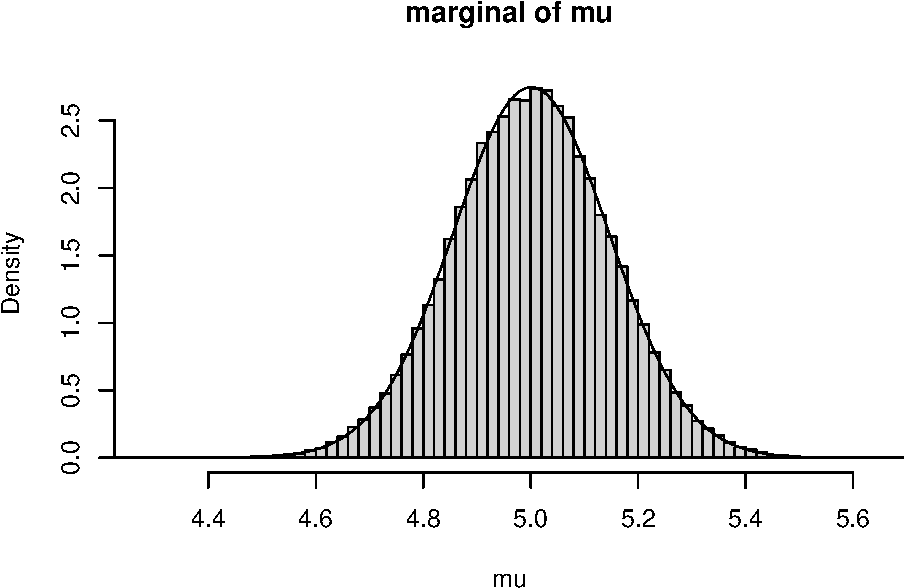
\includegraphics{a_files/figure-latex/unnamed-chunk-25-1.pdf}

\begin{Shaded}
\begin{Highlighting}[]
\FunctionTok{hist}\NormalTok{(tau.dist, }\AttributeTok{freq =}\NormalTok{ F, }\AttributeTok{breaks =} \DecValTok{50}\NormalTok{, }\AttributeTok{main =} \StringTok{"marginal of tau"}\NormalTok{, }\AttributeTok{xlab =} \StringTok{"tau"}\NormalTok{)}
\FunctionTok{lines}\NormalTok{(}\FunctionTok{seq}\NormalTok{(}\FloatTok{0.15}\NormalTok{, }\FloatTok{0.4}\NormalTok{, }\AttributeTok{by =} \FloatTok{0.01}\NormalTok{), }\FunctionTok{dgamma}\NormalTok{(}\FunctionTok{seq}\NormalTok{(}\FloatTok{0.15}\NormalTok{, }\FloatTok{0.4}\NormalTok{, }\AttributeTok{by =} \FloatTok{0.01}\NormalTok{), }\AttributeTok{shape =}\NormalTok{ a }\SpecialCharTok{+}\NormalTok{ x.n}\SpecialCharTok{/}\DecValTok{2}\NormalTok{,}
    \AttributeTok{rate =}\NormalTok{ b }\SpecialCharTok{+}\NormalTok{ x.n }\SpecialCharTok{*}\NormalTok{ (x.s2 }\SpecialCharTok{+}\NormalTok{ (mu.est }\SpecialCharTok{{-}}\NormalTok{ x.mu)}\SpecialCharTok{\^{}}\DecValTok{2}\NormalTok{)}\SpecialCharTok{/}\DecValTok{2}\NormalTok{))}
\end{Highlighting}
\end{Shaded}

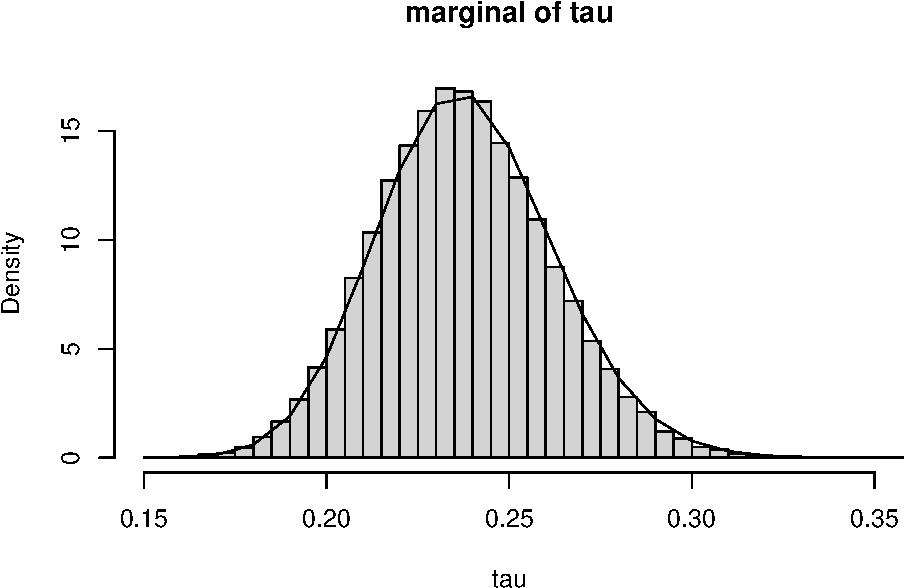
\includegraphics{a_files/figure-latex/unnamed-chunk-25-2.pdf}

\end{document}
